\chapter{Bài toán và dữ liệu}
\section{Mục tiêu}
Mục tiêu là xác định chuyên mục của một bài báo VietnamNet. Thực nghiệm so sánh hai cách khai thác văn bản: các baseline chỉ đọc tiêu đề, còn PhoBERT được fine-tuning với cả tiêu đề và nội dung. Ngoài kết quả chung, báo cáo xem xét các chuyên mục khó phân loại và tác động của hiệu chỉnh xác suất. Mô hình được chọn trên validation rồi đánh giá trên test.

\section{Nguồn và làm sạch dữ liệu}
Bộ dữ liệu VietnamNet News được thu thập bằng crawling từ các trang bài báo công khai của VietnamNet và công bố trên \href{https://huggingface.co/datasets/dathuynh1108/vietnamnet-news}{kho Hugging Face của học viên Huỳnh Thành Đạt} \cite{vietnamnet}. Dữ liệu gồm 212.705 bài báo thuộc 19 chuyên mục, lưu trong 19 tệp Parquet theo chuyên mục. Mỗi bản ghi có bốn trường: \code{title} (tiêu đề), \code{content} (nội dung), \code{url} (đường dẫn bài báo) và \code{class} (nhãn chuyên mục).

Tiêu đề và nội dung được chuẩn hóa Unicode NFC và khoảng trắng. URL được chuẩn hóa, bỏ query và fragment. Các bản ghi có cùng URL, cùng tiêu đề không phân biệt hoa thường hoặc cùng nội dung không rỗng được gộp thành nhóm; Nếu bài A trùng với bài B và bài B trùng với bài C, cả ba được xếp chung nhóm. Nhóm chứa nhiều nhãn chuyên mục bị loại toàn bộ vì chưa có cơ sở xác định nhãn đúng; mỗi nhóm còn lại giữ một bản ghi. Bảng~\ref{tab:text-cleaning} tóm tắt số bài ở từng bước.

\begin{table}[htbp]\centering
\begin{tabularx}{\textwidth}{Xr}\toprule
Bước xử lý & Số bài\\\midrule
Dữ liệu nguồn & 212.705\\
Loại tiêu đề rỗng & 1.167\\
Loại dòng thuộc nhóm có nhãn mâu thuẫn & 3.636\\
Loại dòng trùng còn lại & 527\\
Bài hợp lệ được sử dụng & 207.375\\\bottomrule
\end{tabularx}
\caption{Làm sạch toàn bộ dữ liệu trước khi chia tập. Các số bài bị loại ở ba bước là các phần rời nhau.}
\label{tab:text-cleaning}
\end{table}

Không giới hạn số bài theo chuyên mục. Bảy bài thiếu nội dung vẫn có tiêu đề hợp lệ và được giữ lại. Phân bố sau làm sạch còn mất cân bằng: Sức khỏe có 12.444 bài, còn Dân tộc -- Tôn giáo có 2.917 bài, chênh khoảng 4,27 lần. Accuracy cho biết tỷ lệ bài được phân loại đúng, nhưng có thể che khuất kết quả ở các lớp ít bài. Vì vậy, macro-F1, tức trung bình F1 của 19 lớp với trọng số bằng nhau, được dùng để chọn checkpoint; loss cũng được điều chỉnh theo tần suất lớp trong tập train.

\begin{figure}[htbp]\centering
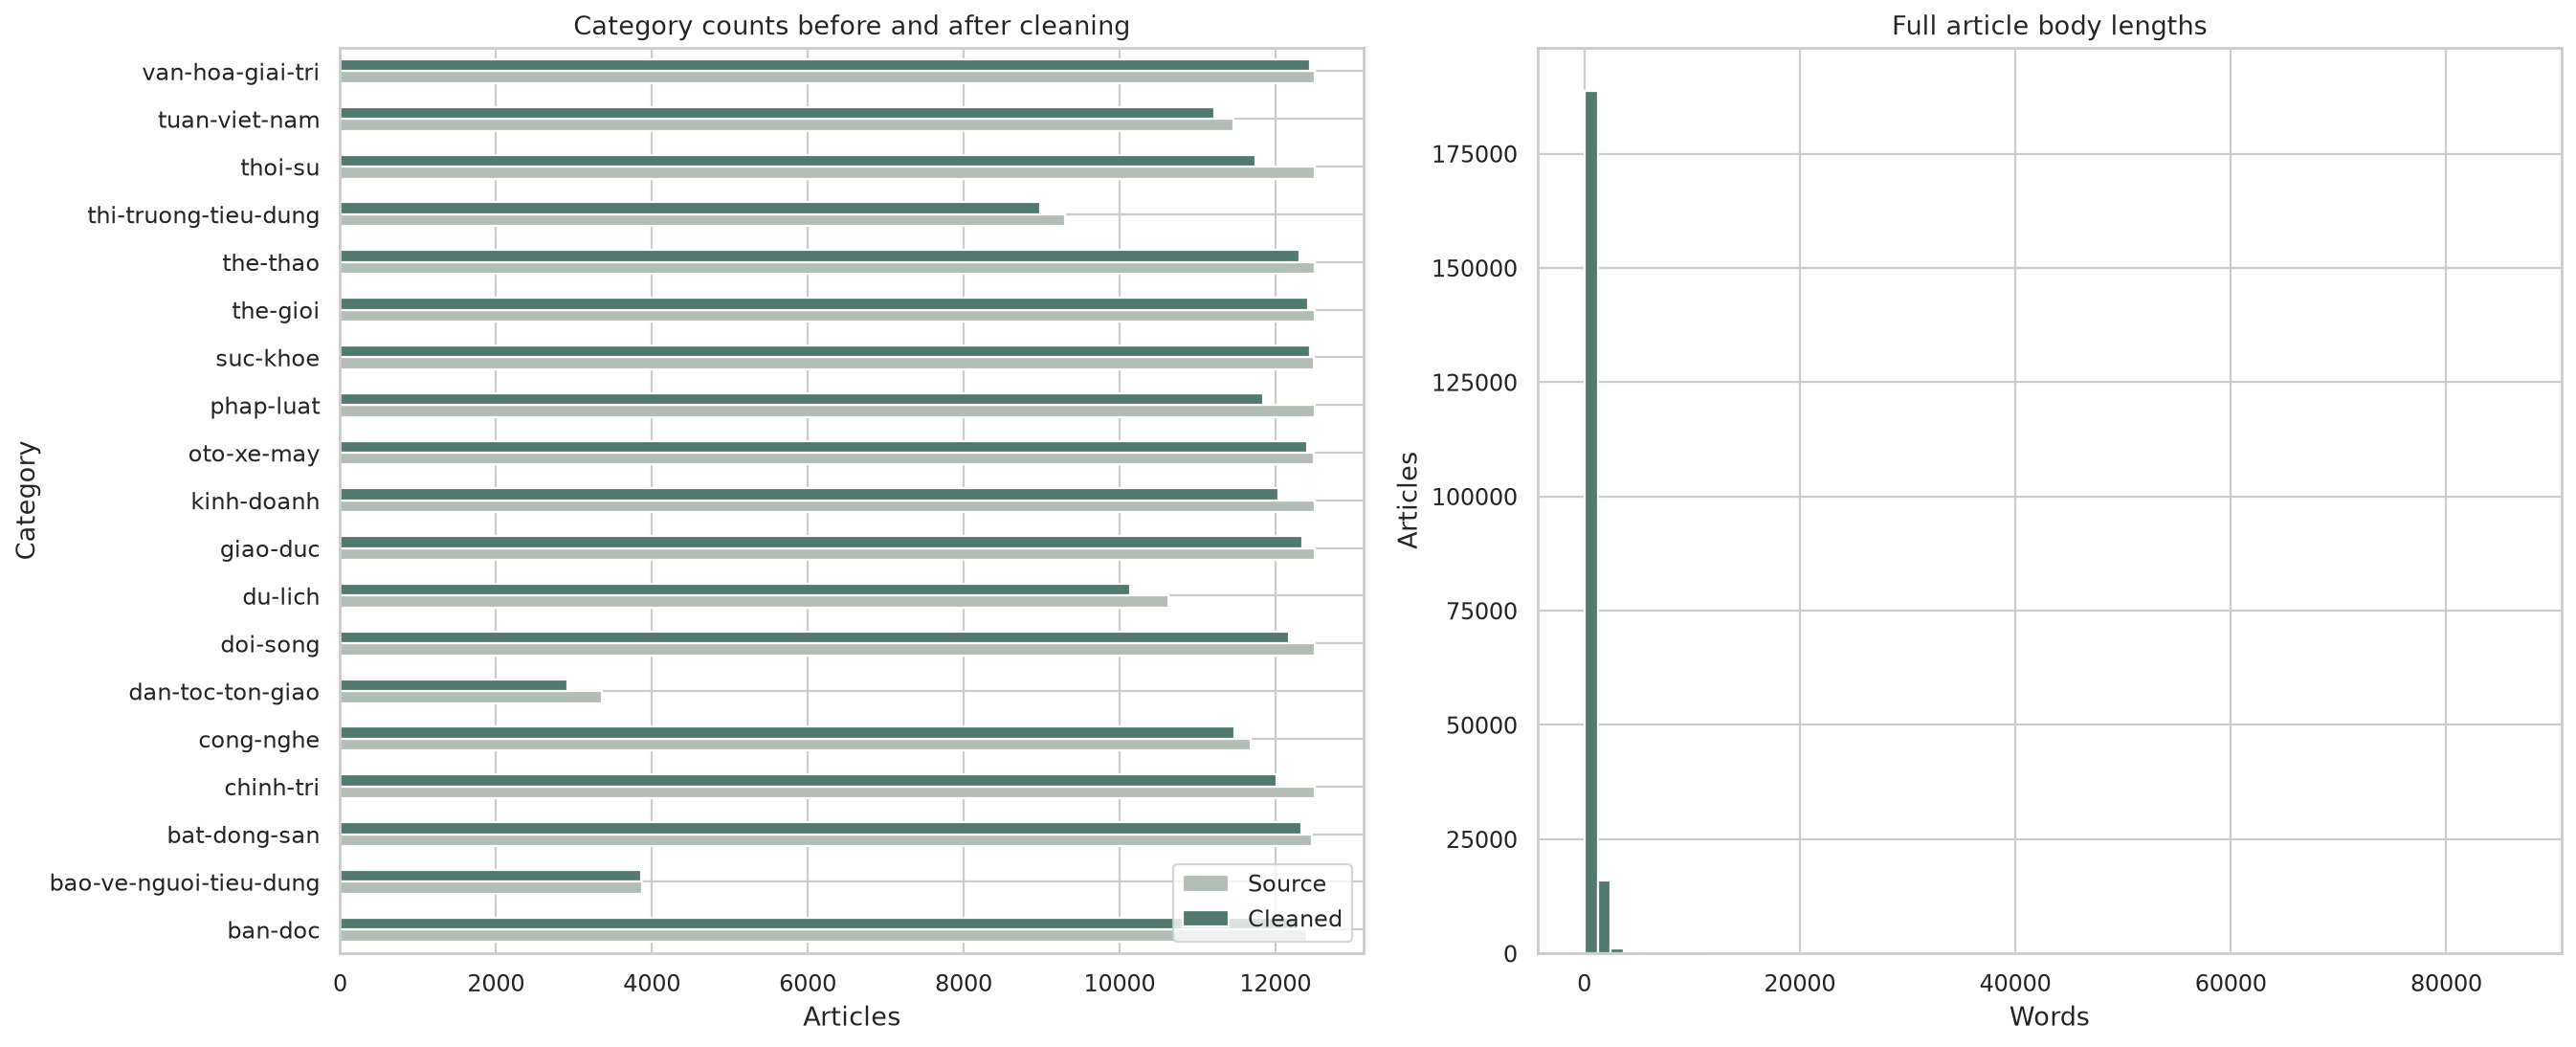
\includegraphics[width=\textwidth]{figures/eda.png}
\caption{Phân bố chuyên mục trước và sau làm sạch, cùng độ dài nội dung trước rút gọn. Toàn bộ bài hợp lệ được sử dụng; sự chênh lệch số mẫu giữa các chuyên mục vẫn được giữ lại.}
\label{fig:text-eda}
\end{figure}

\section{Chia tập theo nhóm đầu vào}
Chuẩn hóa văn bản và giới hạn token có thể khiến các bài khác nhau ở dữ liệu nguồn trở thành cùng một đầu vào mô hình. Vì vậy, các bài có cùng chuỗi token cuối cùng của tiêu đề tối đa 128 token hoặc cùng đầu vào Head--Tail của bài báo 256 token được gộp vào cùng nhóm. Quy tắc gộp nhóm áp dụng cho cả đầu vào của baseline và PhoBERT fine-tuning.

Sau khi gộp, dữ liệu có 207.108 nhóm đầu vào, trong đó 50 nhóm chứa nhiều bài; nhóm lớn nhất có 39 bài. Mọi bài trong cùng nhóm được đưa vào một tập để tránh xuất hiện cùng đầu vào ở cả train và test.

StratifiedGroupKFold chia dữ liệu thành 20 phần với seed 2026, đồng thời giữ phân bố chuyên mục gần nhau giữa các phần. Trong đó, 14 phần dành cho train, ba phần cho validation và ba phần cho test. Ba tập lần lượt có 145.162, 31.107 và 31.106 bài, tương ứng khoảng 70/15/15. Tất cả mô hình dùng chung cách chia này.

\chapter{Phương pháp và thiết lập}
\section{PhoBERT và hàm mất mát}
PhoBERT đã được pretrained trên văn bản tiếng Việt \cite{phobert}. Thực nghiệm dùng PhoBERT Base v2 và bổ sung đầu phân loại 19 lớp theo kiến trúc RoBERTa \cite{phobert-v2}. Encoder biến văn bản thành các vector chứa thông tin ngữ cảnh; đầu phân loại tính một điểm số (logit) cho mỗi chuyên mục. Khi fine-tuning, cả encoder và đầu phân loại đều được cập nhật theo nhãn bài báo.

Để tăng vai trò của các chuyên mục ít bài, cross-entropy sử dụng trọng số lớp tính từ tập train:

\[
w_c=\frac{N_{\mathrm{train}}}{K n_c},\qquad K=19,
\]
trong đó $n_c$ là số bài thuộc lớp $c$ trong tập train. Cross-entropy trên batch $B$ dùng trung bình có trọng số:
\[
\mathcal{L}_B=-\frac{\sum_{i\in B}w_{y_i}\log p_\theta(y_i\mid x_i)}{\sum_{i\in B}w_{y_i}}.
\]
Theo công thức này, một lỗi ở lớp ít bài đóng góp vào loss nhiều hơn một lỗi ở lớp đông bài. Gradient được tích lũy từ hai batch, mỗi batch 32 bài báo, trước khi cập nhật trọng số. Nhờ vậy, mỗi bước cập nhật sử dụng thông tin từ 64 bài mà chỉ cần xử lý 32 bài trên GPU cùng lúc.

\section{Biểu diễn Head--Tail}
Tiêu đề cung cấp thông tin ngắn gọn về bài viết, còn nội dung bổ sung ngữ cảnh khi tiêu đề chưa đủ để xác định chuyên mục. Để giới hạn độ dài xử lý, mỗi đầu vào kết hợp tiêu đề với nội dung bài. Khi nội dung vượt 300 từ, chỉ giữ 220 từ đầu và 80 từ cuối; nội dung ngắn hơn được giữ nguyên. Văn bản được chuyển sang chữ thường, loại dấu câu và chữ số, chuẩn hóa khoảng trắng rồi tách từ bằng PyVi \cite{pyvi}. PhoBERT yêu cầu văn bản đã tách từ trước bước mã hóa subword \cite{phobert-v2}.

Với chuỗi vượt giới hạn đầu vào, Head--Tail giữ 127 subword token đầu và 127 token cuối, kèm hai token đặc biệt:
\[
x=\texttt{<s>}\Vert t_{1:127}\Vert t_{L-126:L}\Vert\texttt{</s>}.
\]
Chuỗi ngắn hơn được bổ sung padding. Attention mask đánh dấu vị trí văn bản thật để mô hình bỏ qua padding. Head--Tail đưa thông tin ở cả đầu và cuối bài vào giới hạn 256 token; đổi lại, phần giữa không được sử dụng. Việc loại chữ số cũng bỏ đi những thông tin như năm, giá tiền hoặc tỷ số.

\section{Huấn luyện và lựa chọn checkpoint}
Mô hình được huấn luyện trong bảy epoch trên toàn bộ tập train. AdamW cập nhật đồng thời encoder và đầu phân loại; learning rate nhỏ giúp điều chỉnh biểu diễn pretrained mà không thay đổi quá mạnh ngay từ đầu. Bảng dưới trình bày các tham số chính.
\begin{table}[htbp]\centering
\begin{tabularx}{\textwidth}{Xl}\toprule
Tham số & Giá trị\\\midrule
Mô hình / số lớp & PhoBERT Base v2 / 19\\
Độ dài đầu vào & 256 token\\
Optimizer & AdamW\\
Learning rate ban đầu & $2\times10^{-5}$\\
Weight decay & 0,01\\
Warmup & 200 bước\\
Batch size & 32 bài báo\\
Gradient accumulation & 2 batch trước mỗi bước cập nhật\\
Batch hiệu dụng & 64 bài báo mỗi bước cập nhật\\
Số epoch & 7\\
Tiêu chí chọn checkpoint & Macro-F1 validation lớn nhất\\
Seed dữ liệu / mô hình & 2026 / 42\\
GPU và kiểu tính toán & RTX 5090, BF16\\\bottomrule
\end{tabularx}
\caption{Thiết lập fine-tuning PhoBERT Base v2 trên VietnamNet trong bảy epoch, với model seed 42.}
\end{table}

Warmup tăng dần learning rate trong 200 bước đầu, giúp đầu phân loại mới bắt đầu học với các cập nhật nhỏ. Sau đó learning rate giảm tuyến tính về 0. Gradient norm được giới hạn ở 1 để hạn chế bước cập nhật quá lớn; bias và tham số LayerNorm không chịu weight decay.

Sau mỗi epoch, mô hình được đánh giá trên validation. Checkpoint có macro-F1 cao nhất được giữ để đánh giá test; khi hòa, giữ checkpoint xuất hiện sớm hơn. Quá trình huấn luyện vẫn thực hiện đủ bảy epoch.

Mô hình hoàn tất bảy epoch với 15.883 bước cập nhật trong 1.506,0 giây, tương đương 25,10 phút. Thời lượng gồm huấn luyện và đánh giá validation sau mỗi epoch, không gồm tải và chuẩn bị dữ liệu. Checkpoint epoch 6 được chọn với macro-F1 validation 0,908943.

\section{Các baseline}
Bốn baseline dùng cùng các bài trong tập train, validation và test với mô hình chính. Đầu vào văn bản của các baseline chỉ gồm tiêu đề:
\begin{itemize}
\item \textbf{Majority baseline:} luôn dự đoán chuyên mục xuất hiện nhiều nhất trong tập train.
\item \textbf{Word TF-IDF + Linear SVM:} biểu diễn tiêu đề bằng TF-IDF theo từ với unigram và bigram, sau đó phân loại bằng SVM tuyến tính.
\item \textbf{Character TF-IDF + Linear SVM:} sử dụng TF-IDF với n-gram ký tự dài 3--5 trong phạm vi từng từ, kết hợp SVM tuyến tính.
\item \textbf{Frozen PhoBERT + Logistic regression:} giữ nguyên trọng số PhoBERT và mã hóa tiêu đề với độ dài tối đa 128 token. Vector đặc trưng 768 chiều được tính bằng trung bình các vector token có attention mask hợp lệ, rồi đưa vào logistic regression.
\end{itemize}

Majority baseline cho biết kết quả khi chỉ dựa vào tần suất nhãn. Hai SVM đánh giá mức độ phân biệt chuyên mục của từ và cụm ký tự trong tiêu đề; Frozen PhoBERT đánh giá biểu diễn pretrained khi encoder chưa được cập nhật theo nhãn chuyên mục. Từ vựng và IDF chỉ được học trên tập train, với tối đa 80.000 đặc trưng cho mỗi biểu diễn TF-IDF. Hệ số $C$ của SVM và logistic regression được chọn trong $\{0{,}5;1;2\}$ theo macro-F1 trên tập validation.

\section{Hiệu chỉnh trên validation}
Với logits $z_{i,c}$, temperature scaling tạo xác suất
\[
p_{i,c}(T)=\frac{\exp(z_{i,c}/T)}{\sum_{k=1}^{K}\exp(z_{i,k}/T)},\qquad T>0.
\]
Negative log-likelihood (NLL) đo mức phạt khi mô hình gán xác suất thấp cho nhãn đúng. Temperature $T$ điều chỉnh độ tập trung của xác suất: $T$ lớn hơn làm xác suất bớt chênh lệch giữa các lớp. Tham số này được chọn trong $[0{,}5;5]$ để giảm negative log-likelihood trên validation. Tiếp theo, mỗi lớp nhận một hệ số $t_c$ để điều chỉnh điểm số tương đối. Hệ số được thử lần lượt cho từng lớp qua hai lượt, với 101 giá trị cách đều trong $[0{,}5;2]$; chỉ giữ thay đổi làm tăng F1 của lớp đó trên validation. Nhãn cuối cùng được chọn theo
\[
\widehat y_i=\arg\max_c\frac{p_{i,c}(T)}{t_c}.
\]
Chia cho $t_c$ nhỏ hơn sẽ tăng điểm tương đối của lớp $c$, nên có thể đổi nhãn dự đoán. Ngược lại, temperature riêng lẻ chỉ đổi độ tự tin và giữ nguyên lớp có điểm cao nhất. Checkpoint, temperature và các hệ số lớp đều được chọn bằng validation trước khi đánh giá trên test.

\chapter{Kết quả và phân tích}
\section{Train loss và kết quả validation theo epoch}
\begin{table}[htbp]\centering
\begin{tabularx}{\textwidth}{rXXX}\toprule
Epoch & Cross-entropy validation có trọng số & Accuracy validation & Macro-F1 validation\\\midrule
1 & 0,3801 & 89,17\% & 0,8810 \\
2 & 0,3242 & 90,57\% & 0,8963 \\
3 & 0,3120 & 90,80\% & 0,8982 \\
4 & 0,3458 & 91,43\% & 0,9063 \\
5 & 0,3572 & 91,37\% & 0,9057 \\
6 & 0,4005 & 91,62\% & 0,9089 \\
7 & 0,4165 & 91,60\% & 0,9084 \\
\bottomrule\end{tabularx}
\caption{Cross-entropy có trọng số lớp, accuracy và macro-F1 validation của PhoBERT Base v2 sau mỗi epoch ở seed 42.}
\label{tab:text-epochs}
\end{table}

Macro-F1 validation đạt cao nhất ở epoch 6 rồi giảm nhẹ ở epoch 7. Trong khi đó, cross-entropy validation thấp nhất ở epoch 3 và tăng về cuối, dù train loss tiếp tục giảm. Mô hình học khớp tập train tốt hơn nhưng không cải thiện tương ứng trên validation.

Hai chỉ số đo các mặt khác nhau: cross-entropy xét xác suất gán cho nhãn đúng, còn F1 xét nhãn được chọn. Vì tiêu chí lựa chọn là macro-F1, checkpoint epoch 6 được dùng cho các bước tiếp theo.

\begin{figure}[htbp]\centering
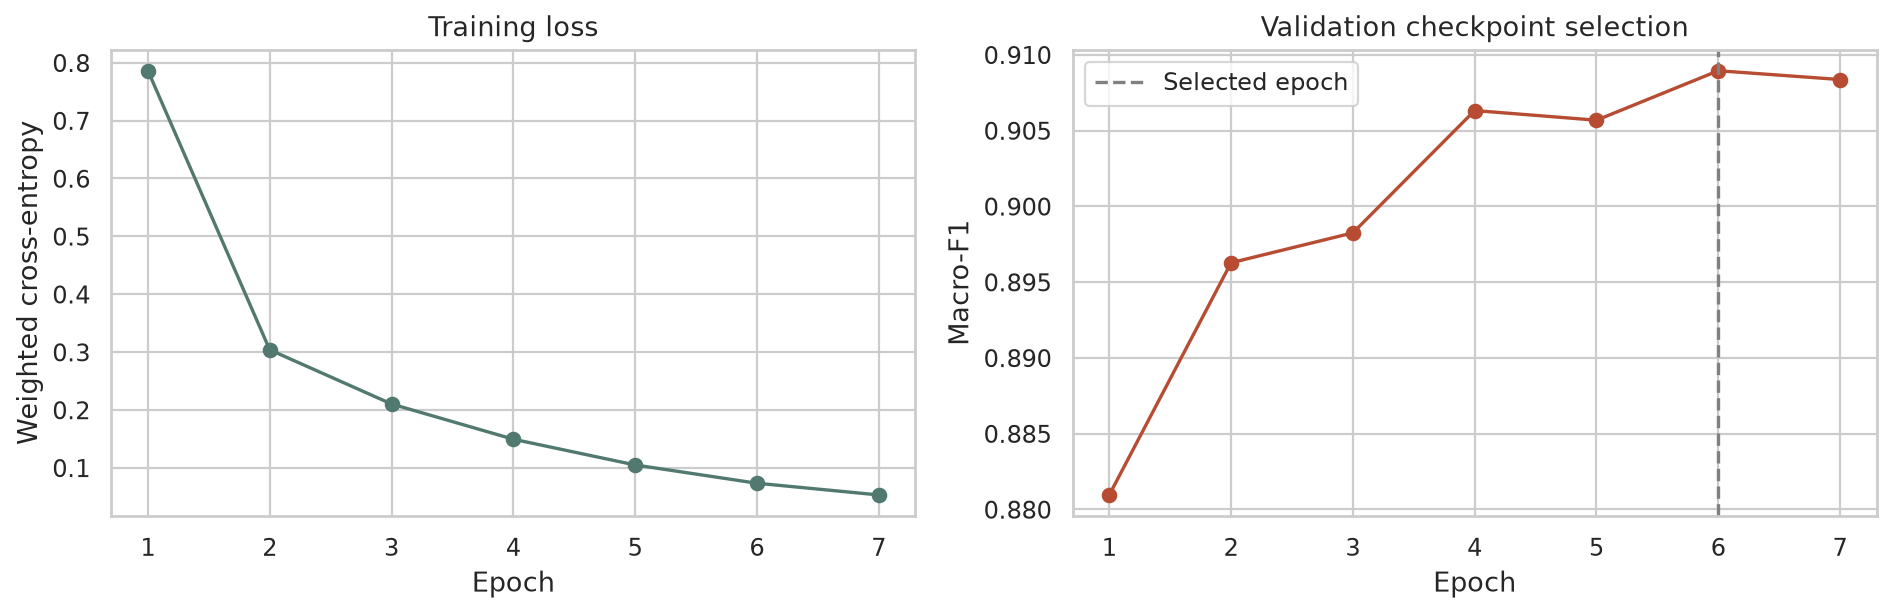
\includegraphics[width=.98\textwidth]{figures/training_curves.png}
\caption{Train loss trung bình và macro-F1 validation của PhoBERT Base v2 qua bảy epoch ở seed 42.}
\end{figure}

\section{Kết quả trên tập test}
\begin{table}[htbp]\centering
\begin{tabularx}{\textwidth}{Xrrr}\toprule
Quy tắc dự đoán & Accuracy & Macro-F1 & Weighted-F1\\\midrule
Argmax logits & 91,7862\% & 0,910280 & 0,917829\\
Temperature và hệ số lớp & 91,7829\% & 0,910362 & 0,917786\\\bottomrule
\end{tabularx}
\caption[Kết quả trước và sau hiệu chỉnh bằng validation]{Accuracy, macro-F1 và weighted-F1 test của PhoBERT Base v2 trước và sau hiệu chỉnh bằng validation, ở seed 42.}
\label{tab:text-results}
\end{table}

Với $T=1,4531$, NLL validation giảm từ 0,3619 xuống 0,3042: xác suất dự đoán bớt tập trung quá mức và phù hợp hơn với nhãn validation. Khi thêm hệ số lớp, macro-F1 test tăng rất nhẹ, còn accuracy và weighted-F1 giảm nhẹ.

Cụ thể, hiệu chỉnh sửa đúng 130 bài nhưng làm sai thêm 131 bài, khiến số bài đúng giảm từ 28.551 xuống 28.550. Như vậy, hiệu chỉnh cải thiện NLL trên validation nhưng chưa mang lại lợi ích phân loại rõ rệt trên test. Các thay đổi nhãn đến từ hệ số lớp, vì temperature riêng lẻ giữ nguyên nhãn argmax.

\section{Chất lượng theo chuyên mục}
\begin{table}[htbp]\centering\small
\begin{tabularx}{\textwidth}{Xrrrr}\toprule
Chuyên mục & Số bài báo & Precision & Recall & F1\\\midrule
Dân tộc -- Tôn giáo & 437 & 0,8131 & 0,7963 & 0,8046 \\
Kinh doanh & 1.806 & 0,8432 & 0,8189 & 0,8309 \\
Thị trường tiêu dùng & 1.347 & 0,8406 & 0,8263 & 0,8334 \\
Đời sống & 1.826 & 0,8368 & 0,8450 & 0,8409 \\
Thời sự & 1.761 & 0,8587 & 0,8626 & 0,8606 \\
Ô tô -- Xe máy & 1.861 & 0,9759 & 0,9812 & 0,9786 \\
Thế giới & 1.863 & 0,9725 & 0,9678 & 0,9701 \\
Thể thao & 1.846 & 0,9876 & 0,9919 & 0,9897 \\
\bottomrule\end{tabularx}
\caption{Precision, recall và F1 test của PhoBERT Base v2 sau hiệu chỉnh ở các chuyên mục có F1 thấp và cao, với seed 42.}
\label{tab:text-classes}
\end{table}

Thể thao được phân loại tốt nhất, còn Dân tộc -- Tôn giáo có F1 thấp nhất. Tuy nhiên, lớp ít bài không phải nguyên nhân duy nhất của kết quả thấp: Kinh doanh có số bài test gần bằng Thể thao nhưng F1 thấp hơn rõ rệt. Điều này gợi ý cần xem thêm ranh giới nội dung giữa các chuyên mục. Weighted-F1 cao hơn macro-F1 cũng cho thấy kết quả tổng hợp thay đổi khi các lớp đông bài được tính trọng số lớn hơn.

\begin{figure}[htbp]\centering
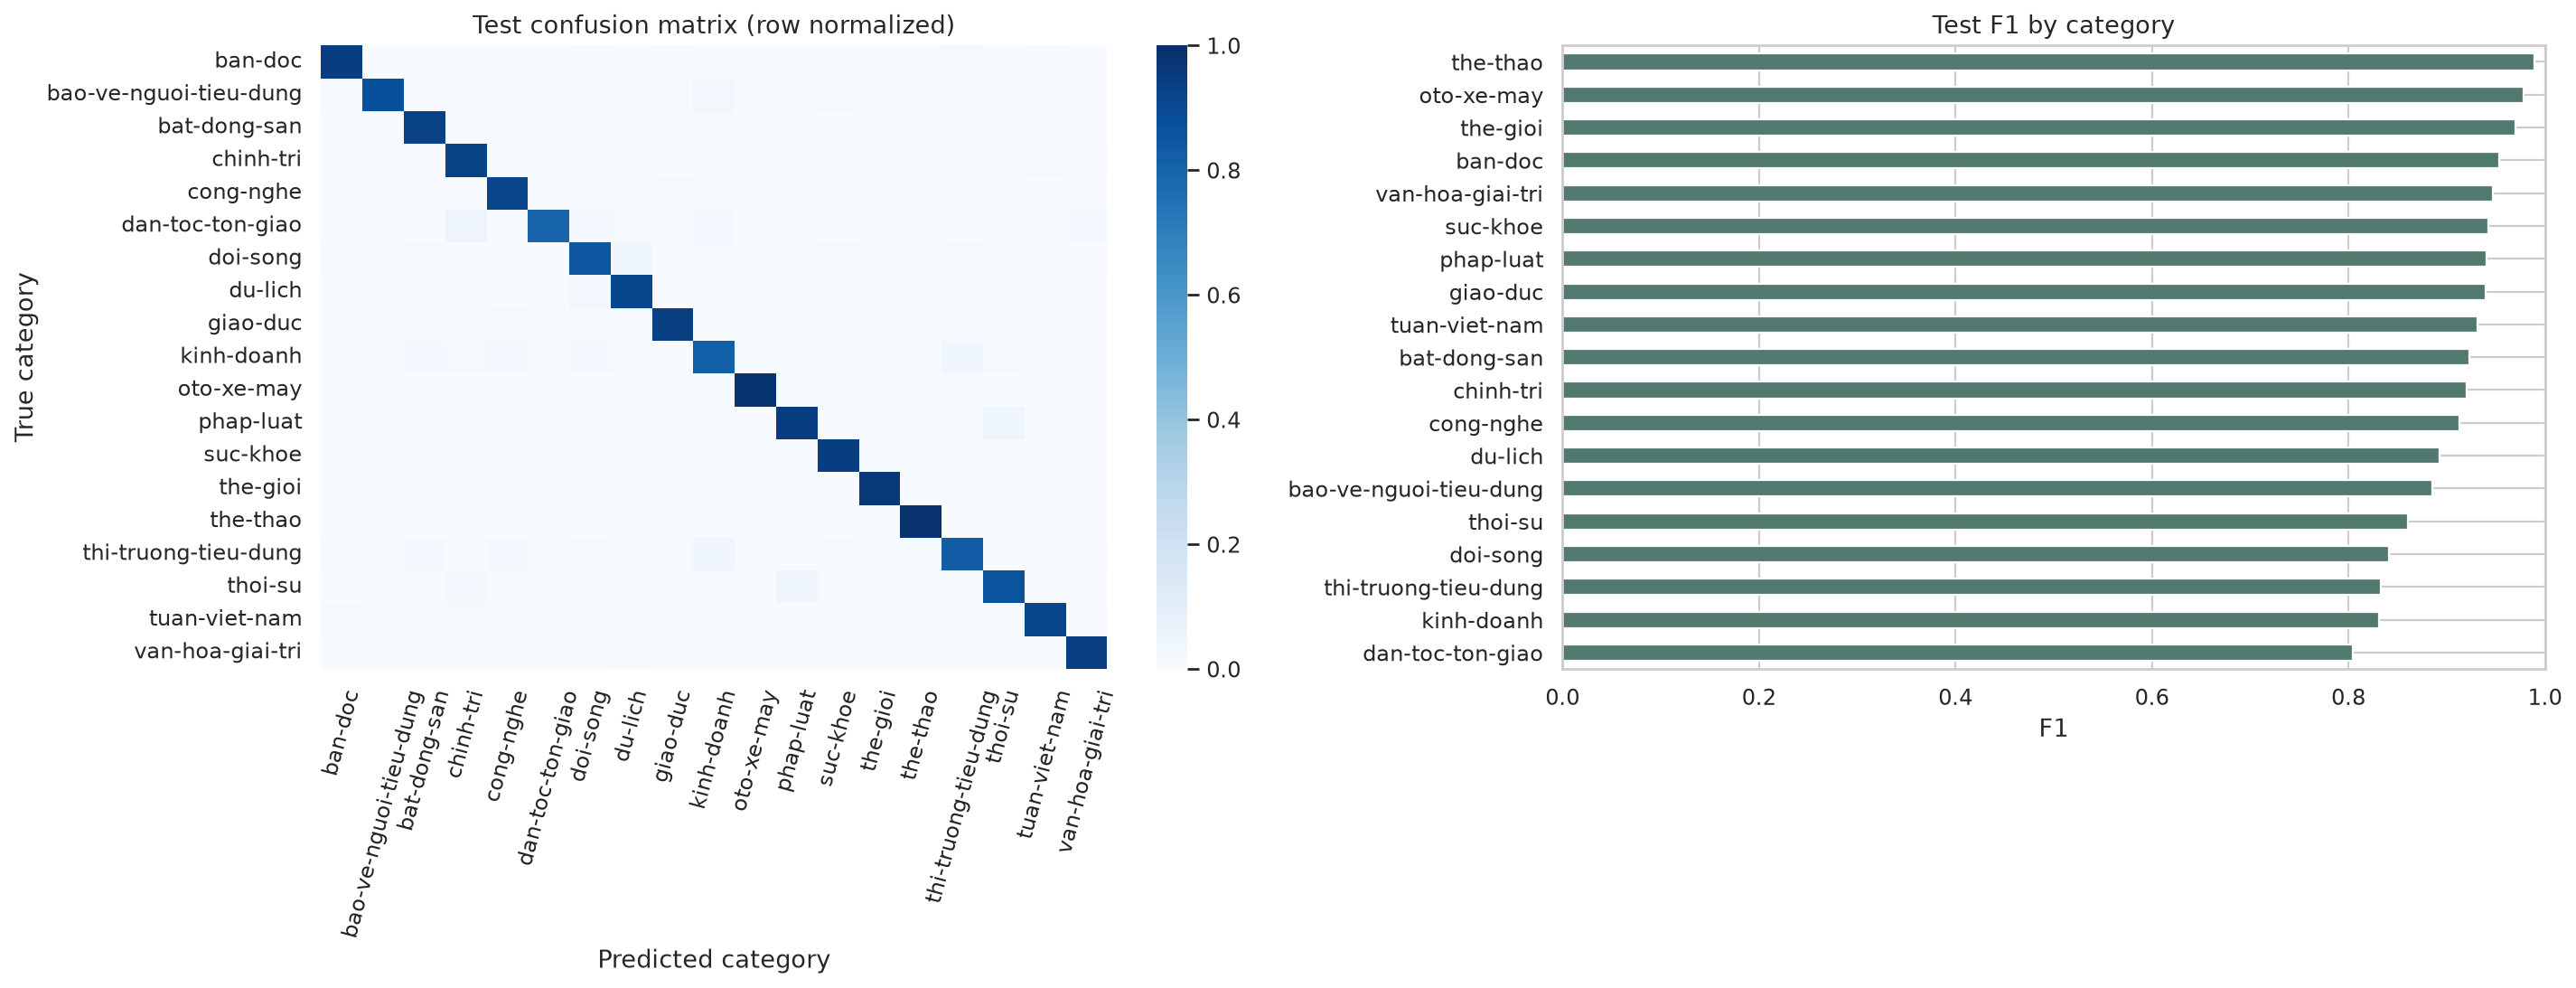
\includegraphics[width=\textwidth]{figures/test_confusion_and_class_f1.png}
\caption{Confusion matrix test chuẩn hóa theo hàng và F1 theo chuyên mục của PhoBERT Base v2 sau hiệu chỉnh ở seed 42. Hàng biểu diễn nhãn thật, cột biểu diễn nhãn dự đoán.}
\label{fig:text-confusion}
\end{figure}

Lỗi phổ biến nhất là dự đoán Thời sự thành Pháp luật, với 89 bài; chiều ngược lại có 78 bài. Đời sống và Du lịch, cũng như Kinh doanh và Thị trường tiêu dùng, là các cặp dễ nhầm khác. Những hướng nhầm lẫn này cho thấy mô hình còn khó phân biệt một số chuyên mục gần nhau. Để xác định nguyên nhân cụ thể, cần đọc lại bài sai cùng nhãn nguồn và phần văn bản được đưa vào mô hình.

\section{So sánh các mô hình}
Frozen PhoBERT + Logistic regression đạt kết quả tốt nhất trong bốn baseline. Hai SVM có chất lượng gần nhau: Character TF-IDF nhỉnh hơn trên test, còn Word TF-IDF nhỉnh hơn trên validation. Vì thứ tự thay đổi giữa hai tập, chưa có ưu thế rõ rệt cho một trong hai cách biểu diễn.

Validation chọn $C=1$ cho logistic regression và $C=0{,}5$ cho cả hai SVM. Kết quả đầy đủ được trình bày trong bảng và hình dưới đây.

\begin{table}[htbp]\centering
\begin{tabularx}{\textwidth}{Xrr}\toprule
Mô hình & Accuracy test & Macro-F1 test\\\midrule
Majority baseline & 6,0021\% & 0,005960\\
Word TF-IDF + Linear SVM & 80,1839\% & 0,783550\\
Character TF-IDF + Linear SVM & 80,2675\% & 0,785815\\
Frozen PhoBERT + Logistic regression & 80,9040\% & 0,793118\\
PhoBERT fine-tuning (argmax) & 91,7862\% & 0,910280\\
PhoBERT fine-tuning + calibration & 91,7829\% & 0,910362\\\bottomrule
\end{tabularx}
\caption[Kết quả các mô hình]{Accuracy và macro-F1 của bốn baseline và PhoBERT Base v2 trên 31.106 bài báo test của VietnamNet, với model seed 42.}
\label{tab:text-headline-comparison}
\end{table}

\begin{figure}[htbp]\centering
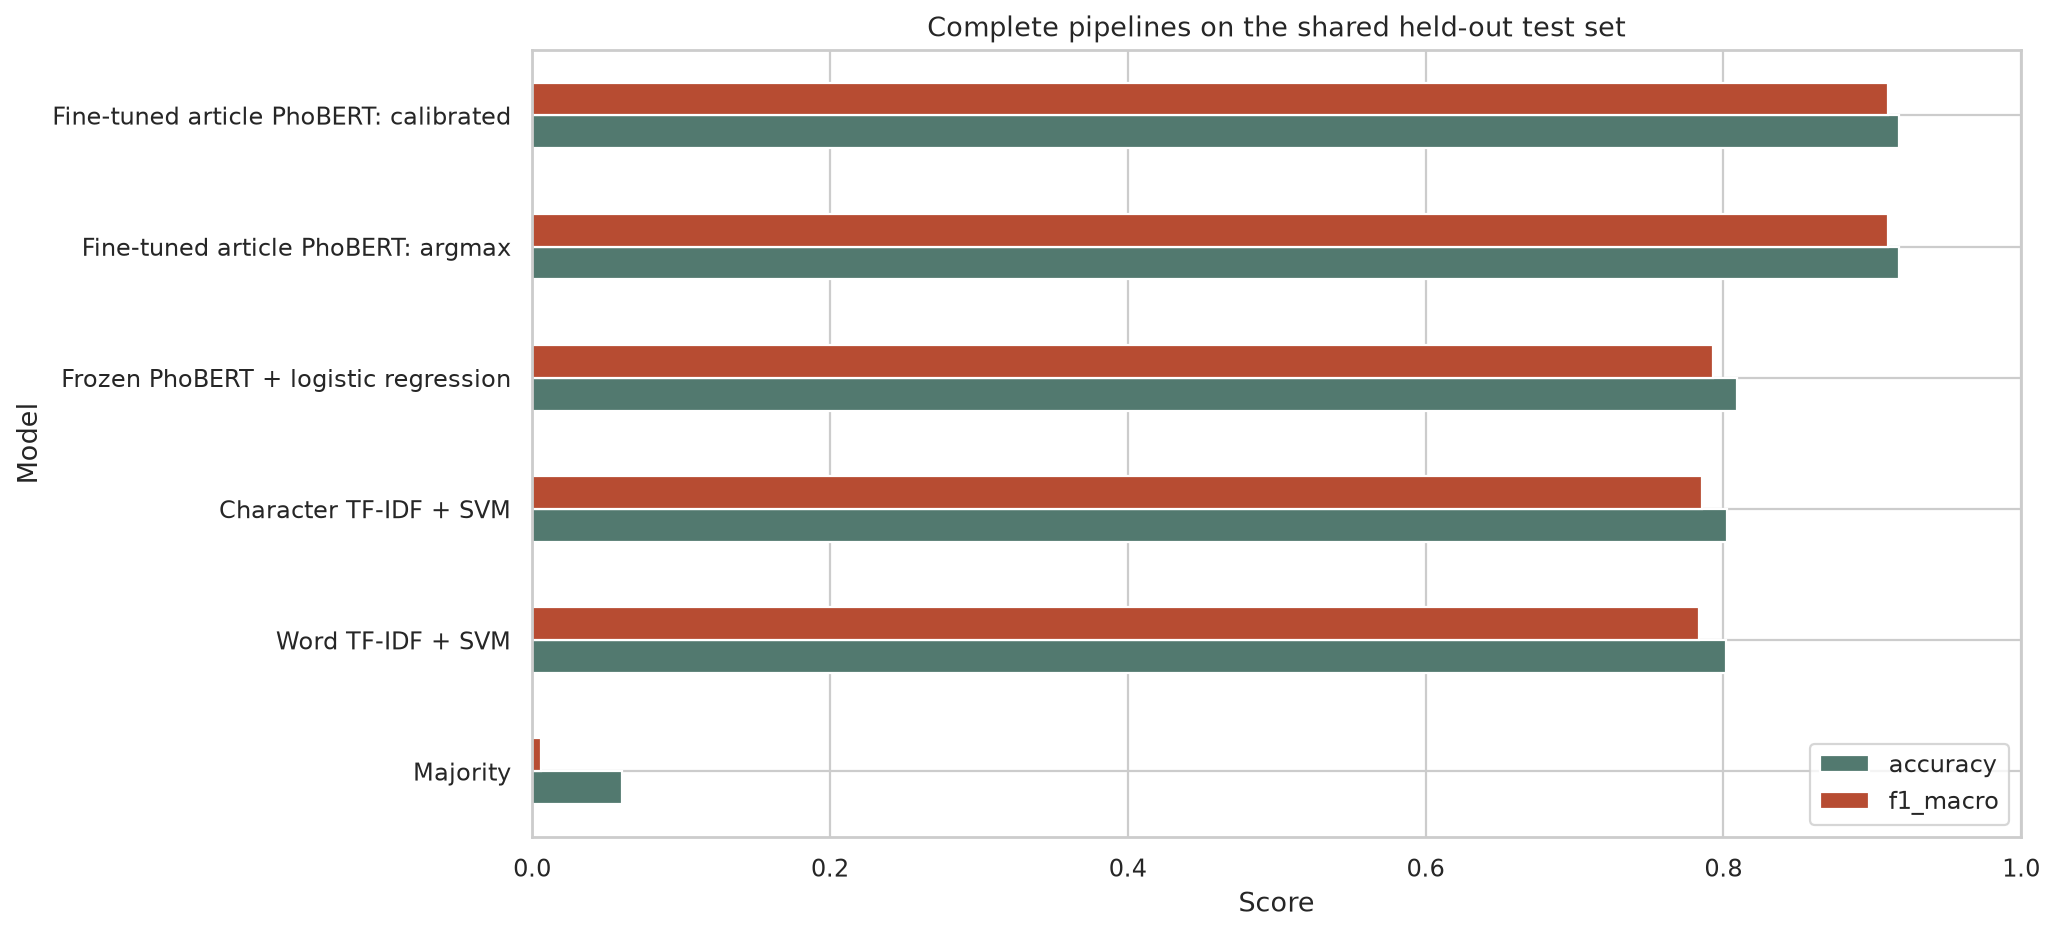
\includegraphics[width=\textwidth]{figures/model_comparison.png}
\caption{Accuracy và macro-F1 của các quy trình trên 31.106 bài báo test ở seed 42. PhoBERT fine-tuning dùng tiêu đề và nội dung đạt accuracy 91,79\%, so với 80,90\% của Frozen PhoBERT dùng tiêu đề.}
\label{fig:text-model-comparison}
\end{figure}

PhoBERT fine-tuning cao hơn baseline Frozen PhoBERT khoảng 10,88 điểm phần trăm accuracy. Kết quả ủng hộ việc khai thác thêm nội dung và điều chỉnh encoder theo chuyên mục. Tuy nhiên, hai phương pháp khác nhau ở cả đầu vào lẫn cách học, nên phép so sánh này chưa xác định riêng mức đóng góp của từng thay đổi.

\chapter{Kết luận và giới hạn}
PhoBERT fine-tuning đạt accuracy 91,79\% trên test và vượt bốn baseline chỉ dùng tiêu đề. Hiệu chỉnh bằng validation làm macro-F1 tăng rất nhẹ nhưng giảm một bài dự đoán đúng, nên không tạo cải thiện phân loại rõ rệt. Chênh lệch giữa các chuyên mục vẫn là vấn đề đáng chú ý hơn mức thay đổi do hiệu chỉnh.

Thực nghiệm sử dụng một cách chia dữ liệu và một seed. Cần chạy thêm để đánh giá độ ổn định, đồng thời xem xét các bài gần trùng về nội dung và khả năng phân loại tin ở thời điểm khác. Hai lựa chọn tiền xử lý cần được đối chiếu riêng là Head--Tail, vốn bỏ phần giữa bài, và loại chữ số. Các hướng này chưa được thực nghiệm trong báo cáo.

Phạm vi hỗ trợ AI được trình bày trong \href{https://github.com/dathuynh1108/CO5177-PFDAV/blob/main/AI_USE_REPORT.md}{AI\_USE\_REPORT.md}.

\begin{thebibliography}{4}\addcontentsline{toc}{chapter}{Tài liệu tham khảo}
\bibitem{vietnamnet} \emph{VietnamNet News}. Dữ liệu thu thập bằng crawling từ VietnamNet, công bố trên kho Hugging Face của học viên Huỳnh Thành Đạt. \url{https://huggingface.co/datasets/dathuynh1108/vietnamnet-news}.
\bibitem{phobert} Dat Quoc Nguyen và Anh Tuan Nguyen. \emph{PhoBERT: Pre-trained language models for Vietnamese}. Trong \emph{Findings of the Association for Computational Linguistics: EMNLP 2020}, tr. 1037--1042, Association for Computational Linguistics, 2020. DOI: \href{https://doi.org/10.18653/v1/2020.findings-emnlp.92}{10.18653/v1/2020.findings-emnlp.92}. \url{https://aclanthology.org/2020.findings-emnlp.92/}.
\bibitem{phobert-v2} VinAI Research. \emph{PhoBERT Base v2 model card}. \url{https://huggingface.co/vinai/phobert-base-v2}.
\bibitem{pyvi} PyVi 0.1.1. \emph{Vietnamese word segmentation}. \url{https://pypi.org/project/pyvi/}.
\end{thebibliography}
